% \documentclass{report}

% \usepackage{subcaption} % package for subfigures
% \usepackage{hyperref}  % package for linking figures etc
% \usepackage{enumitem}  % package for description with bullets
% \usepackage{graphicx}  % package for importing images
% \usepackage{mathtools} % package for math equation
% \usepackage{mathrsfs}  % package for math font
% \usepackage{indentfirst} % package for getting ident after section or paragraph
% \usepackage[export]{adjustbox}
% \usepackage{longtable} % package for multi pages tables
% \usepackage{multirow}  % package for tables, multirow
% \usepackage{esvect}
% % \usepackage{amsmath}

% \setlength{\parindent}{2em} % how much indent to use when we start a paragraph

% \graphicspath{ {./theory/figures/} }       % path for images

% \begin{document}

\chapter{Classification stage}
\textbf{Pending introduction...}
\section{Description}
After getting all proposed tubes, it's time to do classification. As classifiers we use several approaches including a Linear Classifier, 
a Recursive Neural Network (RNN) Classifier, a Support Vector Machine (SVM) Classifier and a Multilayer perceptron (MLP).

\begin{figure}[h]
  % 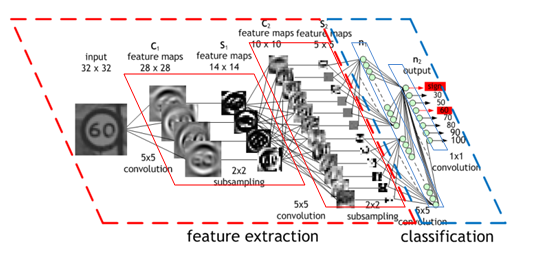
\includegraphics[scale=0.7]{convolutional_neural_network_structure} \]
  \centering
  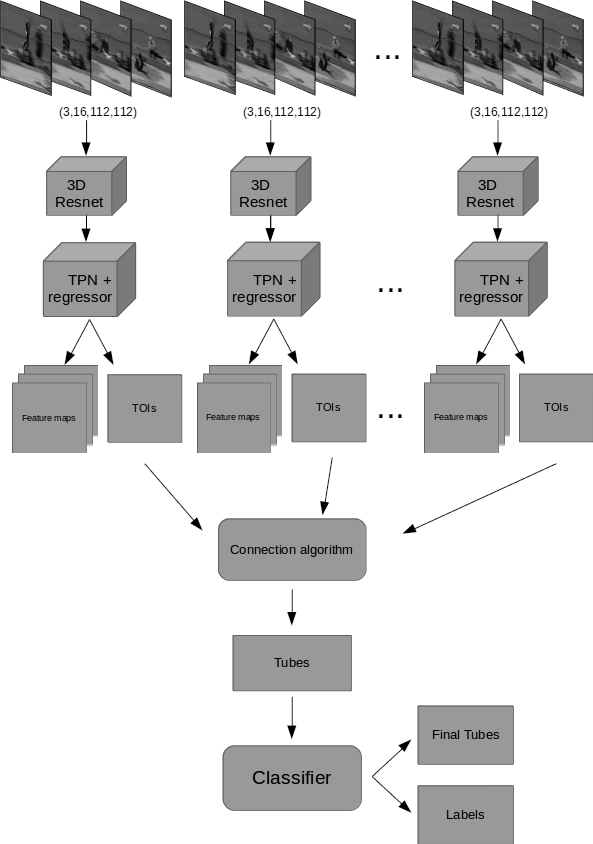
\includegraphics[scale=0.42]{model_withoutnms_v2}
  \caption{Structure of the whole network}
  \label{fig:whole_network}
\end{figure}

The whole procedure of classification is consisted from the following steps:
\begin{enumerate}
\item Separate video into small video clips. Feed TPN network those video clips and get as output
  k-proposed ToIs and their corresponding features for each video clip.
\item Connect the proposed ToIs in order to get video tubes which may contain an action.
\item For each candidate video tube, which is a sequence of ToIs, feed it into the classifier
  for verification.
\end{enumerate}

The general structure of the whole network is depicted in figure \ref{fig:whole_network}, in which we can see the aforementioned steps if we
follow the arrows.  \par
In first steps of classification stage we refer only to JHMDB dataset because it has smaller number of video than UCF dataset which
helped us save a lot of time and resources. That's because  we performed most experiments only JHMDB and after we found the optimal
situation, we implemented to UCF-dataset, too. 

\section{Preparing data  and first classification results}

% \textbf{(Pending... Introduction about Linear and RNN classifiers)}
% \textbf{(Pending.. also an image of RNN classifier)}
For carrying out classification stage, we use, at first, a Linear classifier and a RNN classifier.
\paragraph{Linear Classifier} Linear classifier is a type of classifier which is able to discriminate objects and predict their
class based on the value of a \textit{linear combination} of object's feature values, which usually are presented in a feature
vector. If the input feature vector to the classifier is a real vector  $\vv{x}$, then the output score is :
\[ y = f(\vv{w} \cdot \vv{x}) = f \left( \sum_j w_jx_i \right) \]
\paragraph{RNN}
Recurrent neural networks, or RNNs for short, are a type of neural network that was designed to learn from sequence data,
such as sequences of observations over time, or a sequence of words in a sentence.
RNN takes many input vectors to process them and output other vectors.
It can be roughly pictured like in the Figure \ref{fig:rnn} below,
imagining each rectangle has a vectorial depth and other special hidden quirks in the image below.
For our case, we choose \textbf{many to one} approach, because we want only one prediction, at the end of
the action tube. \par
\begin{figure}[h]
  \centering
  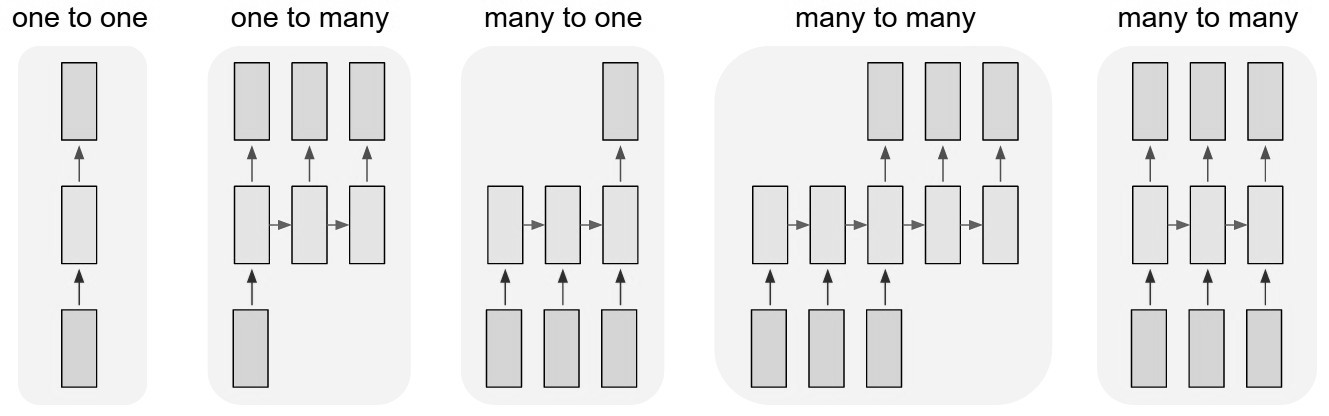
\includegraphics[width=1.\textwidth]{rnn.jpeg}
  \caption{Types of RNN}
  \label{fig:rnn}
\end{figure}

\paragraph{Training}
In order to train our classifier, we have to execute the previous steps for each video. However, each video
has different number of frames and reserves too much memory in the GPU. In order to deal with this situation,
we give as input one video per GPU. So we can handle 4 videos simultaneously. This means that a regular
training session takes too much time for just 1 epoch. \par
The solution we came with, is to precompute the features for both positive video tubes and negative video tubes and 
then to feed those features to our classifier for training  it in order to discriminate classes. This solution includes the following steps:
\begin{enumerate}
\item  At first, we extract only groundtruth video tubes' features and the double number of background video tubes. We chose this
ratio between positive and negative tubes inspired by \cite{jjfaster2rcnn}, in which it has 0.25 ratio between foreground
and background rois and chooses 128 roi in total. Respectively, we chose a little bigger ratio because we have only 1 groundtruth
video tube in each video. So, for each video we got 3 video tubes in total, 1 for positive and 2 for background. We considered
background tubes those whose overlap scores with groundtruth tubes are $ \ge 0.1 $ and $ \le 0.3 $. Of course, we use a pre-trained TPN
in order to get those action tubes.
\item After extracting those features, we trained both Linear and RNN classifiers. The Linear classifier needs a fixed input size, so
  we used a pooling function in the dimension of the videos. So, at first we had a feature map of \textit{3,512,16} dimensions and then
  we get as output a feature maps of \textit{512,16} dimensions. We used both max and avg pooling as shown at Table \ref{table:rnn_linear}.
  For the RNN classifier, we do not use any pooling function before feeding it.
\end{enumerate}
In order to train our classifiers, we use Cross-Entropy Loss as training loss function.
\paragraph{Validation} Validation stage includes using both pre-trained TPN and classifier. So, for each video,
we get classification scores for proposed action tubes. Most approaches usually consider a confidence score for
considering an action tube as foreground. However, we don't use any confidence score. On the contrary, because we
know that JHMDB has trimmed videos with only 1 performed action, we just consider the best-scoring tube as our prediction.


\begin{table}[h]
  \centering
  \begin{tabular}{|| c | c || c  c  c ||}
    \hline
    \multirow{2}{*}{\textbf{Classifier}} & \multirow{2}{*}{\textbf{Pooling}} &  {} & \textbf{mAP} & {} \\
    {} & {} & 0.5 & 0.4 & 0.3 \\
    \hline
    \multirow{2}{*}{Linear} & mean & 14.18 & 19.81 & 20.02 \\
    \cline{2-5}
    {} & max & 13.67 & 16.46 & 17.02 \\
    \hline
    RNN  & -  & 11.3 & 14.14 & 14.84 \\
    \hline
  \end{tabular}
  \caption{First classification results using Linear and RNN classifiers}
  \label{table:rnn_linear}
\end{table}

  
% \textbf{(Pending results RNN... Table)}
% \textbf{(Pending results RNN... commentary)}
Table \ref{table:rnn_linear} shows first classification results, which are not very good. The only useful deduction that we can come with, using above results is that, avg pooling
method outclass max pooling. So, for all the rest classifications using Linear classifier, we use avg pooling before classification
stage.
% The results are disappointing.
% As we can see in the table, RNN classifier cannot classify very well because, probably, the duration of the videos are so small
% so we stopped using it in jHMDB dataset. In the Linear classifier, we noticed that every tube is considered as background tube.
% That means that Linear classifier gets overfitted with trained data and cannot handle unknown data. So, we thought that we
% need a classifier which can \"learn\" very easily, with little data. So we chose to try a support vector machine classifier.

\section{Support Vector Machine (SVM)}
SVMs are classifiers defined by a separating hyper-plane between trained data in a N-dimensional space. The main advantage of using a SVM
is that can get very good classification results when we have few data available. \par
The use of SVM is inspired from \cite{Girshick:2015:FR:2919332.2920125} and it is trained using hard negative mining. 
This means that we have 1 classifier per class which has only 2 labels, positive and negative. We mark as positive the feature maps of the
groundtruth action, and as negative groundtruth actions from other classes, and feature maps from background classes.
As we know, SVM is driven by small number of examples near decision boundary. Our goal is to find a set of negatives that are the closest to
the separating hyper-plane. So in each iteration, we update this set of negatives adding those which our SVM didn't perform very well. Each
SVM is trained independently. \par
SVM code is take from Microsoft's Azure \href{https://github.com/Azure/ObjectDetectionUsingCntk} {github page} in which there is an implementation
of Fast RCNN using a SVM classifier. We didn't modify its parameters which means that it has a linear kernel, uses  L2-norm as penalty and L1-norm
as loss during training. Also, we consider as hard-negatives the tubes that got score $ >  -1.0 $ during classification.\par
This whole process makes the choice of the negatives a crucial factor. In order to find the best policy,  we came with 5 different cases to consider
as negatives:
\begin{enumerate}
\item Negatives are other classes's positives and all the background tubes
\item Negatives are only all the background videos
\item Negatives are only other classes's positives
\item Negatives are other classes's positives and background tubes taken only from videos that contain a positive tube
\item Negatives are only background tubes taken from videos that contain a positive tube
\end{enumerate}

On top of that, we use 2 pooling functions in order to have a fixed input size. \par
In the next tables, we show our architecture's  mAP performance when we follow each one of the above policies. Also,
we experimented for 2 feature maps, \textit{(64,8,7,7)} and \textit{(256,8,7,7)} where 8 equals with the sample duration.
Both feature maps were extracted by using 3D RoiAlign procedure from feature maps with dimensions \textit{(64,8,28,28)} and
\textit{(256,8,7,7)} respectively (in the second case, we just add zeros in the feature map outsize from the bounding boxes for
each frame). Table \ref{table:svm_first_results} contains the first classification results. At first column we have the dimensions
of feature maps before pooling function, where k = 1,2,..5 . At second column we have feature maps' dimensions after pooling, and at
the next 2 column, the type of pooling function and the policy we followed. Finally in the last 3 columns we have the mAP performance
when we have threshold equal with 0.3, 0.4 and 0.5 respectively. During validation, we keep only the best scoring tube because we know that
we have only 1 action per video.

\begin{center}
\begin{longtable}{||c | c | c| c||c c c||}

  \hline
  \multicolumn{2}{||c|}{\textbf{Dimensions}} & \multirow{2}{*}{ \textbf{Pooling}} &\multirow{2}{*}{\textbf{Type}} & \multicolumn{3}{|c||}{\textbf{mAP precision}}\\

   before & after &  {} & {} &  0.5 &  0.4 & 0.3 \\
 \hline   \hline
 \multirow{5}{*}{(k,64,8,7,7)} & \multirow{5}{*}{(1,64,8,7,7)} & \multirow{5}{*}{mean}  & 1 &  3.16 & 4.2 & 4.4    \\
  \cline{4-7}
  {} & {} & {} & 2 & 2.29 & 2.68 & 2.86    \\
    \cline{4-7}
  {} & {} & {} & 3 & 1.63 & 3.16 &  4  \\
    \cline{4-7}
  {} & {} & {} & 4 & 2.42 & 4.83 & 5.46  \\  
    \cline{4-7}
  {} & {} & {} & 5 & 0.89 &1.12 & 1.21  \\
  \hline
 \multirow{5}{*}{(k,64,8,7,7)} & \multirow{5}{*}{(1,64,8,7,7)} & \multirow{5}{*}{max}  & 1 & 1.11 & 2.35 & 2.71 \\
    \cline{4-7}
  {} & {} & {} & 2 & 2.31 & 2.62 & 2.64 \\
    \cline{4-7}
  {} & {} & {} & 3 & 1.11 & 2.35 & 2.71 \\
    \cline{4-7}
  {} & {} & {} & 4 & 1.41 & 2.76 & 3.84  \\
    \cline{4-7}
  {} & {} & {} & 5 & 0.33 & 0.51 &0.58  \\

  \hline   \hline

 \multirow{5}{*}{(k,256,8,7,7)} & \multirow{5}{*}{(1,256,8,7,7)} & \multirow{5}{*}{mean}  & 1 &  11.41 & 11.73 & 11.73 \\

    \cline{4-7}
  {} & {} & {} & 2 & 10.35 & 10.92 &11.89 \\
    \cline{4-7}
  {} & {} & {} & 3 & 8.93 & 9.64 & 9.94 \\
    \cline{4-7}
  {} & {} & {} & 4 & 12.1 & 13.04 &13.04 \\
    \cline{4-7}
  {} & {} & {} & 5 & 5.92 & 6.92 & 7.79 \\
    \hline
 \multirow{5}{*}{(k,256,8,7,7)} & \multirow{5}{*}{(1,256,8,7,7)} & \multirow{5}{*}{max}  & 1  & \textbf{22.07} & \textbf{24.4} &  \textbf{25.77} \\
    \cline{4-7}
  {} & {} & {} & 2  & 14.07 & 16.56 & 17.74 \\
    \cline{4-7}
  {} & {} & {} & 3  & 14.22 & 18.94 &21.6 \\
    \cline{4-7}
  {} & {} & {} & 4  & 21.05 & 24.63 & 25.93 \\
    \cline{4-7}
  {} & {} & {} & 5  & 11.6 & 13.92 & 15.81 \\
  \hline   
  
  \caption{Our architecture's performance using 5 different policies and 2 different feature maps while pooling in
  tubes' dimension. With bold is the best scoring case}
  \label{table:svm_first_results}

\end{longtable} 
\end{center}

From the above results we notice that features map with dimension (256,8,7,7) outperform in all cases, both for mean and max pooling and
for all the policies. Also, we can see that max pooling outperforms mean pooling in all cases, too. Last but not least, we notice that policies
2, 3 and 5 give us the worst results which means that svm needs both data from other classes positives and from background tubes. 

\subsection{Modifying 3D Roi Align}
As we mentioned before, we extract from each tube its activation maps using 3D Roi Align procedure and we set equal to zero the pixels outside
of bounding boxes for each frame. We came with the idea that the environment surrounding the actor sometimes help us determine the class
of the action which is performed. This is base in the idea that 3D Convolutional Networks use the whole scene in order to classify the action
that is performed. We thought to extend a little each bounding box both in width and height. So, during Roi Align procedure, after resizing
the bounding box into the desired spatial scale  ( in our case 1/16 because original sample size = 112 and resized sample size = 7 )
we increase by 1 both width and height. According to that if we have a resized bounding box $( x_1,y_1,x_2,y_2) $ our new bounding box becomes
$ (max(0,x_1-0.5),max(0,y_1-0.5),min(7,x_2+0.5),min(7,y_2+0.5)) $ ( we use \textit{ min} and \textit{max} functions in order to avoid exceeding feature maps' limits).
We just experiment in policies 1 and 4 for both (256,8,7,7) and (64,8,7,7) feature maps as show in  Table \ref{table:svm_mod_roialign}


\begin{center}
\begin{longtable}{||c | c | c| c||c c c||}

  \hline
  \multicolumn{2}{||c|}{\textbf{Dimensions}} & \multirow{2}{*}{ \textbf{Pooling}} &\multirow{2}{*}{\textbf{Type}} & \multicolumn{3}{|c||}{\textbf{mAP precision}}\\

   before & after &  {} & {} &  0.3 &  0.4 & 0.5 \\
 \hline   \hline
 \multirow{2}{*}{(k,64,8,7,7)} & \multirow{2}{*}{(1,64,8,7,7)} & \multirow{2}{*}{mean}  & 1 & 9.75 & 11.92 & 13.34 \\
  \cline{4-7}
  {} & {} & {} & 4 &  5.74 &6.62 & 7.59 \\
  \hline
 \multirow{2}{*}{(k,64,8,7,7)} & \multirow{2}{*}{(1,64,8,7,7)} & \multirow{2}{*}{max}  & 1 &  6.46 & 10.26 & 10.83 \\
    \cline{4-7}
  {} & {} & {} & 4 & 4.19 & 6.27 & 7.52 \\
    \cline{4-7}
  \hline
  \caption{Our architecture's performance using 2 different policies and 2 different pooling methods using modified Roi Align.}
  \label{table:svm_mod_roialign}

\end{longtable} 
\end{center}

According to Table \ref{table:svm_mod_roialign}, modified Roi Align doesn't improve mAP performance. On the contrary, it reduces it.
However, the gap between those 2 approaches is small, so we don't abandon this idea, because, for different approaches,
modified Roi Align may outclass regular Roi Align.

\subsection{Temporal pooling}
After getting first results, we implement a temporal pooling function inspired from \cite{DBLP:journals/corr/HouCS17}. We need a
fixed input size for the SVM. However, our tubes' temporal stride varies from 2 to 5. So we use as fixed temporal pooling equal
with 2. As pooling function we use 3D max pooling, one for each filter of the feature map.  So for example, for an action tube
with 4 consecutive ToIs, we  have 4,256,8,7,7 as feature size. We separate the feature map into 2 groups using \textit{linspace}
function and we reshape the feature map into 256,k,8,7,7 where k is the size of each group, After using 3D max pooling, we get
a feature map 256,8,7,7 so finally we concat them and get 2,256,8,7,7. In this case we didn't experiment with (64,8,7,7) feature
maps because it wouldn't performed better that (256,8,7,7) feature maps as noticed from the previous section. \par
We experiment using a SVM classifier for training policies 1 and 4 and using both regular and modifier Roi Align. The
performance results are presented at Table \ref{table:svm_temp_pooling}.

\begin{center}
\begin{longtable}{||c | c| c| c||c c c||}

  \hline
 \multicolumn{2}{||c|}{\textbf{Dimensions}} & \multirow{2}{*}{\textbf{Pooling}} &\multirow{2}{*}{ \textbf{Type}} &\multicolumn{3}{|c||}{\textbf{mAP precision}}\\

  before & after & {} & {} & 0.5 &  0.4 & 0.3\\
  \hline   \hline

  \multirow{4}{*}{k,256,8,7,7} & \multirow{4}{*}{2,256,8,7,7} & \multirow{2}{*}{RoiAlign}  & 1 & 25.07 & 26.91 & 29.11 \\
  \cline{4-7}
  {} & {} & {} & 4 &  23.27 & 25.96 & 28.25 \\
  \cline{3-7}
  {} & {} & \multirow{2}{*}{mod RoiAlign} & 1 & 7.01 & 9.69 & 10.52 \\
  \cline{4-7}
  {} & {} & {} & 4 & 5.5 & 7.25 & 8.99 \\
  \hline

  \caption{mAP results using temporal pooling for both RoiAlign approaches}
  \label{table:svm_temp_pooling}
\end{longtable} 
\end{center}

Comparing Tables \ref{table:svm_mod_roialign} and \ref{table:svm_temp_pooling}, we clearly notice that we get better results when
using temporal pooling. Also, the difference between regular Roi Align and modified Roi Align become much bigger than previously,
so this makes us abandon the idea of modified Roi Align. So, the rest section, we only experiment using regular Roi Align.

\section{Increasing sample duration to 16 frames}

Next, we though that a good idea would be to increase the sample duration from 8 frames to 16 frames. We experiment both using and not
using temporal pooling, again for policies 1 and 4. Results are included at table \ref{table:svm_temp_pooling_16}. 

\begin{center}
\begin{longtable}{||c | c| c| c||c c c||}

  \hline
 \multicolumn{2}{||c|}{\textbf{Dimensions}} & \multirow{2}{4.5em}{\textbf{Temporal Pooling}} &\multirow{2}{*}{ \textbf{Type}} &\multicolumn{3}{|c||}{\textbf{mAP precision}}\\

  before & after & {} & {} &  0.5 &  0.4 & 0.3 \\
  \hline   \hline

  \multirow{2}{*}{k,256,16,7,7} & \multirow{2}{*}{1,256,16,7,7} & \multirow{2}{*}{No}  & 1 & 23.4 & 27.57 &28.65  \\
  \cline{4-7}
  {} & {} & {} & 4 & 22.7 & 26.95 & 28.05 \\
  \hline

  \multirow{2}{*}{k,256,16,7,7} & \multirow{2}{*}{2,256,16,7,7} & \multirow{2}{*}{Yes}  & 1 & 21.12 & 24.07 & 24.36  \\
  \cline{4-7}
  {} & {} & {} & 4 & 18.36 & 23.09 & 23.75 \\
  \hline
  \caption{mAP results for  policies 1,4  for sample duration = 16 }
  \label{table:svm_temp_pooling_16}
\end{longtable} 
\end{center}

As shown at Table \ref{table:svm_temp_pooling_16}, we get better performance when we don't use temporal pooling, fact that is unexpected.
However, the difference between those performances is about 2\%. Probably, this is caused by the fact that, in the temporal pooling approach,
SVM classifier has to train too many parameters when it uses temporal pooling, on the contrary with the approach not using temporal pooling,
in which SVM has to train half the number of parameters. Furthermore, comparing above results with results shown at Table  \ref{table:svm_mod_roialign}, we can see that we get about the same results for both approaches. So, we choose to keep using approach with sample duration equal
with 8. That's because, we don't have to use too much memory during training and validation.

\section{Adding more groundtruth tubes}
% \textbf{Pending more comments...} \\
% From above results, we notice that SVM improve a lot the performance of our model. In order to further improve our results, we will
% add more groundtruth action tubes. We consider as groundtruth action tubes all the tubes whose overlap score  with a groundtruth tube is
% greater that 0.7 . Also, we increase the total number of tube to from 1 to 2, 8. Table \ref{table:svm_increased}

The previous results came from when we train classifiers using only 1 groundtruth action tube and 2 background. We thought that we should
experiment with the number of foreground action tubes and the ratio between foreground and background tubes because in previous approaches
these numbers were a little arbitraly. So, we choose to train our previous classifiers using 2, 4 and 8 foreground tubes and a ratio of 2:3,
1:2, 1:3, and 1:4 between the number of foreground tubes and the total number of both foreground and background tubes. \par

Firstly, we train the RNN classifier using feature maps with dimensions \textit{(256,8,7,7)} and mAP performance is presented at Table 
\ref{table:rnn_increased} for overlap threshold equal with 0.5, 0.4 and 0.3 . 
% \begin{table}[h]
%   \centering
%   \begin{tabular}{|| c | c | c || c c c||}

\begin{center}
  \begin{longtable}{|| c | c | c || c c c||}
    \hline
    \multirow{2}{*}{\textbf{F. map}} & \multirow{2}{*}{\textbf{FG tubes}}  & \multirow{2}{*}{\textbf{Total tubes}} & {} & \textbf{mAP} & {} \\
    {}  & {} & {} & 0.5 & 0.4 & 0.3 \\
    \hline
    \multirow{7}{*}{(k,256,8,7,7)} & 1 & 3 & 11.3 & 14.14 & 14.84 \\
    \cline{2-6}
    {} & \multirow{4}{*}{2} & 3 & 1.96 & 5.07 & 7.27 \\
    \cline{3-6}
    {} & {} & 4  & 3 & 5.03 & 5.77 \\
    \cline{3-6}
    {} & {} & 6 & 1.34 & 3.89 & 4.49 \\
    \cline{3-6}
    {} & {} & 8 & 0.77 & 1.51 & 2.72 \\
    \cline{2-6}
    {} & \multirow{4}{*}{4} &  6 & 13.23 & 21.74 & 25.4 \\
    \cline{3-6}
    {} & {} & 8 & 20.73 & 28.25 & 29.50 \\
    \cline{3-6}
    {} & {} & 12  & 16.55 & 24.35 & 25.22 \\
    \cline{3-6}
    {} & {} & 16  & 20.11 & 25.50 & 27.62 \\
    \cline{2-6}
    {} & \multirow{4}{*}{8} & 12 & 13.82 & 19.93 & 22.80 \\
    \cline{3-6}
    {} &  {} & 16 & 15.47 & 23.08 & 24.19 \\
    \cline{3-6}
    {} &  {} & 24 & 15.88 & 23.44 & 24.48  \\
    \cline{3-6}
    {} &  {} & 32 &  12.66 & 23.50 & 25.61 \\
    \hline

  \caption{RNN results }
  \label{table:rnn_increased}
\end{longtable}
\end{center}

According to Table \ref{table:rnn_increased}, firstly we can see that increasing the number of foreground tubes from 1 to 2 leads to reduce
rapidly mAP performance. But, when we set foreground tubes equal to 4 we get better results. On top of that, we get best performance when
the ratio is equal with 1:2 and 1:4. Finally, when we set the number of foreground tubes equal with 8, performance gets slightly better
comparing with the initial number and ratio but, this situation doesn't get us the best resutsl. \par 
Next, it's time to experiment using the Linear classifier. We use again the same cases like we did for RNN classification. As mentioned
before, we need a pooling method before classification step. According to Table \ref{table:rnn_linear}, avg pooling method results in
better mAP performance than max pooling, so we use avg pooling for all following cases. Results are included at Table \ref{table:linear_increased}.

\begin{center}
  \begin{longtable}{|| c | c | c || c c c||}
    \hline
    \multirow{2}{*}{\textbf{F. map}} & \multirow{2}{*}{\textbf{FG tubes}} & \multirow{2}{*}{\textbf{Total tubes}} & {} & \textbf{mAP} & {} \\
    {}  & {} & {} & 0.5 & 0.4 & 0.3 \\
    \hline
    \multirow{7}{*}{(k,256,8,7,7)}  & 1 & 3& 14.18 &19.81 & 20.02 \\
    \cline{2-6}
    {} & \multirow{4}{*}{2} & 3 & 12.68 & 13.38 & 15.14 \\
    \cline{3-6}
    {} & {} & 4 & 11.5 & 14.95 & 16.22 \\
    \cline{3-6}
    {} & {} & 6 & 10.74 & 13.36 & 15.18 \\
    \cline{3-6}
    {} & {} & 8 & 8.00 & 9.83 & 11.17 \\
    \cline{2-6}
    {} & \multirow{4}{*}{4} & 6 & 15 & 17.55 & 19.39 \\
    \cline{3-6}
    {} & {} & 8 & 17.04	& 20.12 &22.07 \\
    \cline{3-6}
    {} & {} & 12 & 17.57 & 19.9 & 21.88 \\
    \cline{3-6}
    {} & {} & 16 & 14.24 & 17.24 & 17.95 \\

    \cline{2-6}
    {} & \multirow{4}{*}{8} & 12 & 17.91 & 22.51 & 24.62 \\
    \cline{3-6}
    {} & {} & 16 & 16.76 & 20.34 & 22.72 \\
    \cline{3-6}
    {} & {} & 24 & 17.61 & 19.12 & 24.48 \\
    \cline{3-6}
    {} & {} & 32 & 14.45 & 18.07 & 19.14  \\
    \hline

    \caption{Linear results }
    \label{table:linear_increased}
  \end{longtable}
\end{center}

First of all, after considering results presented at both Tables \ref{table:rnn_increased} and \ref{table:linear_increased}, it becomes clear that when we
set the number of foreground tubes equal with 2, for both case, we get worse results that the initial. This probably is due to the fact that we increase
also the number of background tubes for cases when ratio is 1:2, 1:3 and 1:4 resulting in considering more proposed tubes as background tubes. On the other
hand when we set ratio equal with 2:3, instead of considering most proposed action tubes as background, classifiers classify them as a specific action class,
which means there is an overfitting situation. \par
After considering aforementioned results, for the remaining SVM classifier, we will \textbf{Pending... for case 2}

\begin{center}
  \setlength{\tabcolsep}{2pt}
  \begin{longtable}{|| c | c | c || c c c||}


    \hline
    \multirow{2}{*}{\textbf{F. map}} & \multirow{2}{*}{\textbf{FG tubes}} & \multirow{2}{*}{\textbf{Total tubes}} & {} & \textbf{mAP} & {} \\
    {}  & {} & {} & 0.5 & 0.4 & 0.3 \\
    \hline
    \multirow{8}{*}{(2,256,8,7,7)} & 1 & 3 & 25.07 & 26.91 & 29.11\\
    \cline{2-6}
    {} & \multirow{4}{*}{2} & 3 & Pending... \\
    \cline{3-6}
    {} & {} & 4 & Pending... \\
    \cline{3-6}
    {} & {} & 6 &  Pending... \\
    \cline{3-6}
    {} & {} & 8 & Pending... \\
    \cline{2-6}
    {} & \multirow{4}{*}{4} & 6 & Pending... \\
    \cline{3-6}
    {} & {} &  8 & 24.34 & 25.67 & 26.34 \\
    \cline{3-6}
    {} & {} & 12 &  23.47 & 25.31 & 25.9 \\
    \cline{3-6}
    {} & {} & 16 & 21.94 & 23.55 & 24.23 \\
    \cline{2-6}
    {} & \multirow{4}{*}{8} & 12 & Pending...\\
    \cline{3-6}
    {} & {} & 16 & 23.97 & 26.38 & 26.94 \\
    \cline{3-6}
    {} & {} & 24 & 24.17 & 26.24 & 26.76 \\
    \cline{3-6}
    {} & {} & 32 & 24.17 & 26.24 & 26.76 \\

    \hline

    \caption{SVM results }
    \label{table:svm_increased}
  \end{longtable}
\end{center}
\textbf{Pending... commentary}

\subsection{Increasing again sample duration (only for RNN and Linear)}

Table \ref{table:svm_temp_pooling_16} showed that SVM classifier gets about the same performance for both sample durations 8 and 16 frames.
Triggered by this fact, we trained RNN and Linear classifiers for sample duration equal with 16 frames. Table \ref{table:rnn_16} shows RNN's mAP
performance and Table \ref{table:linear_16} Linear's mAP performance.

\begin{center}
  \begin{longtable}{|| c | c || c c c ||}
    \hline
    \multirow{2}{*}{\textbf{FG tubes}} & \multirow{2}{*}{\textbf{Total tubes}} & {} & \textbf{mAP} & {} \\
    {} & {} & 0.5 & 0.4 & 0.3 \\
    \hline
    \multirow{4}{*}{4} & 6 & Pending...\\
    \cline{2-5}
    {} & 8 & 10.88 & 14.02 & 14.74  \\
    \cline{2-5}
    {} & 12 & 14.05 & 19.23 & 20.99 \\
    \cline{2-5}
    {} & 16 & 11.69 & 15.77 & 16.87  \\
    \hline
    \multirow{4}{*}{8} & 12 & Pending...\\
    \cline{2-5}
    {} & 16 &  12.29 & 19.51 & 23.11  \\
    \cline{2-5}
    {} & 24 & 12.85 & 18.35 & 20.00 \\
    \cline{2-5}
    {} & 32 & 9.38 & 14.33 & 16 \\
    \hline

  \caption{RNN results for sample duration equal with 16}
  \label{table:rnn_16}
\end{longtable}
\end{center}

\begin{center}
  \begin{longtable}{|| c | c || c c c ||}
    \hline
    \multirow{2}{*}{\textbf{FG tubes}} & \multirow{2}{*}{\textbf{Total tubes}} & {} & \textbf{mAP} & {} \\
    {} & {} & 0.5 & 0.4 & 0.3 \\
    \hline
    \multirow{4}{*}{4} & 6 & Pending...\\
    \cline{2-5}
    {} & 8 & 15.11 & 19.78 & 21.14 \\
    \cline{2-5}
    {} & 12 & 11.39 & 15.74 & 18.15 \\
    \cline{2-5}
    {} & 16 & 13.62 & 16.11 & 18.15 \\
    \hline
    \multirow{4}{*}{8} & 12 & Pending...\\
    \cline{2-5}
    {} & 16 & 12.98 & 17.52 & 19.10 \\
    \cline{2-5}
    {} & 24 & 12.92 & 17.64 & 19.95 \\
    \cline{2-5}
    {} & 32 & 11.51 & 13.98 & 14.82 \\
    \hline

  \caption{Linear results for sample duration equal with 16}
  \label{table:linear_16}
\end{longtable}
\end{center}

\textbf{ Pending... commentary}

\section{MultiLayer Perceptron (MLP)}

\begin{figure}[h]
  % 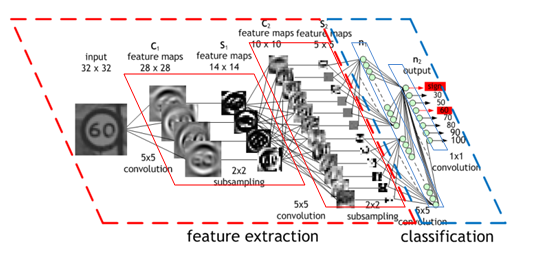
\includegraphics[scale=0.7]{convolutional_neural_network_structure} \]
  \centering
  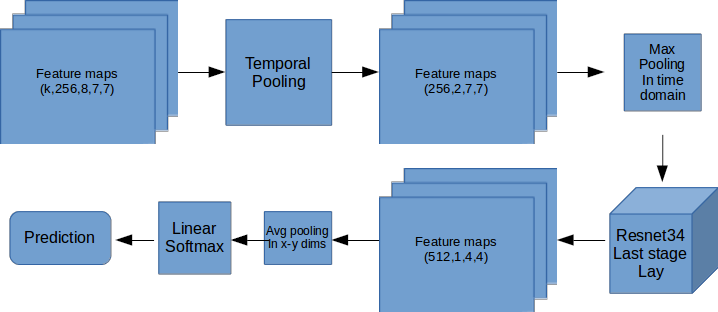
\includegraphics[scale=0.42]{mlp}
  \caption{Structure of the MLP classifier}
  \label{fig:mlp_structure}
\end{figure}

In previous sections we used classic classifiers like Linear, RNN and SVM. Last but not least approach,
another widely category of classifiers  is Multilayer Perceptorn (MLP) classifiers. MLP is a class of
feedforward Neural Network, so its function is described in chapter 2.
So, we design a MLP which is shown in Figure \ref{fig:mlp_structure} for sample duration equal with 8, and is described below:
\begin{itemize}
\item At first,  after 3D Roi align and for sample duration = 8, we get an activation map of $(k,256,8,7,7)$ where $k$ is the
  number of linked ToIs. Inspired by previous sections, we perform temporal pooling followed by a max pooling operation in
  sample duration's dimension. So, we now have an activation maps with dimensions equal with $(2,256,7,7),$ which we reshape
  it into $(256,2,7,7).$ 
 we extracted layers from the last stage of ResNet34. This stages includes 3 Residual Layers
  with stride equal with 2 in all 3 dimensions and output number of filters equal with 512.

\item After Residual Layers, we perform temporal pooling for x-y dimensions. So we get as output activation maps with dimension size
  equal with (512,).  Finally, we feed these feature maps to a linear layer in order to get class confidence score, after applying
  soft-max function.

\end{itemize}

\subsection{Regular training}
According to figure \ref{fig:whole_network}, the trainable parts of our network is TPN and the classifier.
% At first, we tried to
% simultaneously train them, but, we got OutOfMemory errors during training, even thought we tried several modifications in our code.
% So, we came with the idea of, first training seperately TPN, according to chapter 4 and then train the whole network by freezeing
% TPN's layers. 
As mentioned before, training code requires running only one video per GPU, because, videos have different duration. For previous approaches
we came with the idea of pre-calculating video features and then training only the classifier. However, for this step, we normally trained our
in order to get classification results. Of course, we used a pre-trained TPN, whose layers were freezed in order not to be trained.
We tried to explore different ratios between the number of foreground tubes and the total number of tubes per video. First 3 simulations included
fixed number of total tubes and variable ratio between the number of foreground and background tubes. We started using only foreground tubes, which
means 32 out 32 tubes are foreground, then half of the proposed tubes aka 16 out of 32 and finally less than half, namely 14 out of 32. After that,
we experiment using a fixed number of foreground tubes and variable number of total tubes, which are 16, 24 and 32. The performance results are presented
at Table \ref{table:mlp_reg}.

\begin{center}
  \begin{longtable}{|| c | c || c c c ||}
    \hline
    \multirow{2}{*}{\textbf{FG tubes}} & \multirow{2}{*}{\textbf{Total tubes}} & {} &  \textbf{mAP} & {} \\
    {} & {} & 0.5 & 0.4 & 0.3 \\
    \hline
    32 & \multirow{3}{*}{32} &1.28 & 1.73 & 1.87  \\
    \cline{1-1} \cline{3-5}
    16 & {} & 3.98 & 4.38 & 4.38  \\
    \cline{1-1} \cline{3-5}
    14 & {} & 0.40 & 0.40 & 0.40 \\
    \hline
    \multirow{3}{*}{8} & 16 & 9.41 & 12.59 & 14.61 \\
    \cline{2-5}
    {} & 24 & 12.32 & 15.53 & 18.57 \\
    \cline{2-5}
    {} & 32 & 7.16 & 10.92 & 13.00 \\
    \hline
    \caption{MLP'smAP performance for regular training procedure}
    \label{table:mlp_reg}
  \end{longtable}
\end{center}

The results show that when first 3 approaches give us very bad results. Comparing them with the rest 3, we came with the conclusion that we
need at the most 8 foreground tubes, even thought the ration between the number of foreground and background is in favor the second one.
Probably, too many foreground action tubes make our architecture overfitted so unable to generalize.

\subsection{Extract features}
\textbf{Pending...}
As previously performed, we trained MLP classifier using pre-computed feature maps. These feature maps include both foreground and background
action tubes. Base on the conclusion made in previous sections, we will train our classifier only for number of foreground tubes equal with 4
and 8. Furthermore, we will train it for 3 different ratios between the number of foreground and background action tubes, which are 1:1, 1:2
and 1:3. Table \ref{table:mlp_extract_jhdmb} shows these cases and their respective mAP performance during validation step.

\begin{center}
  \begin{longtable}{|| c | c || c c c ||}
    \hline
    \multirow{2}{*}{\textbf{FG tubes}} & \multirow{2}{*}{\textbf{Total tubes}} & {} & \textbf{mAP} & {} \\
    {} & {} & 0.5 & 0.4 & 0.3 \\
    \hline
    \multirow{3}{*}{4} & 6 & Pending...\\
    \cline{2-5}
    {} & 8 & 5.89 & 9.54 & 13.61 \\
    \cline{2-5}
    {} & 12 & 9.51 & 12.8 & 14.6  \\
    \cline{2-5}
    {} & 16 & 6.80 & 13.17 & 14.67 \\
    \hline
    \multirow{4}{*}{8} & 12 & Pending...\\
    \cline{2-5}
    {} & 16 & 8.49 & 13.94 & 15.09 \\
    \cline{2-5}
    {} & 24 & 6.72 & 12.17 & 15.30 \\
    \cline{2-5}
    {} & 32 & 13.27 & 17.64 & 18.97 \\
    \hline

  \caption{mAP results for MLP trained using extracted features}
  \label{table:mlp_extract_jhdmb}
\end{longtable}
\end{center}

\textbf{Pending.. commentary}

\section{Adding nms algorithm}

After getting previous classification results, we came with the idea that a lot of proposed action tubes overlap spatiotemporally like presented in chapter 4,
for the first linking algorithm. On top of that, even though, at last, we will keep only the best scoring action tube, maybe, our Network sometimes
doesn't score the best overlapping action tube but a neighbour, which should have been removed. So, similar with chapter 4, we added NMS algorithm
before classification stage in order to remove unnecessary overlapping action tubes.
The structure of this approach is presented at Figure \ref{fig:network_nms}. So, we run again validation stage for our classifiers
and results are presented at Tables \ref{table:svm_nms}, \ref{table:rnn_nms}, \ref{table:linear_nms} and \ref{table:mlp_nms} for SVM, RNN, Linear
and MLP classifiers respectively.

\begin{figure}[h]
  % 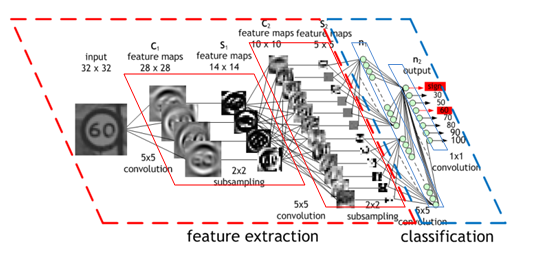
\includegraphics[scale=0.7]{convolutional_neural_network_structure} \]
  \centering
  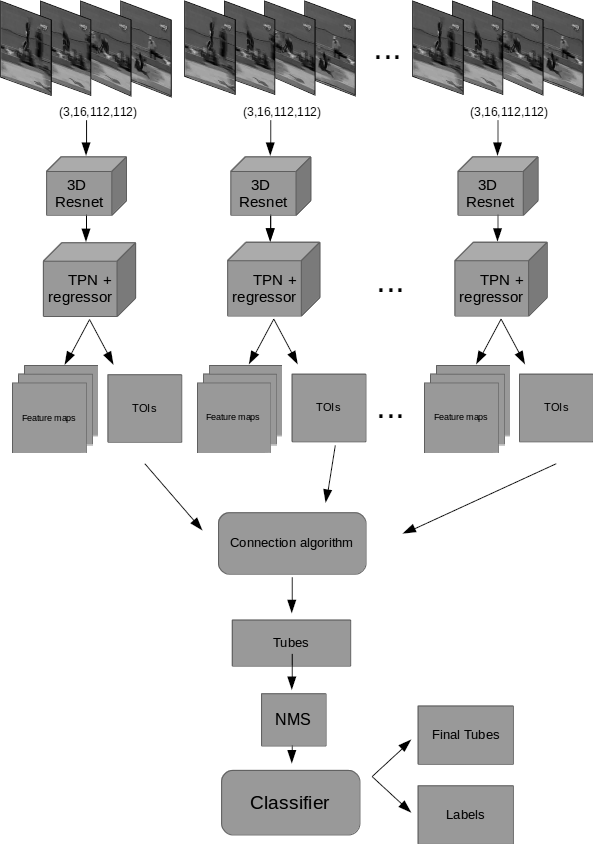
\includegraphics[scale=0.4]{model_withnms}
  \caption{Structure of the network with NMS}
  \label{fig:network_nms}
\end{figure}

\begin{center}
  \begin{longtable}{|| c | c || c c c ||}
    \hline
    \multirow{2}{*}{\textbf{FG tubes}} & \multirow{2}{*}{\textbf{Total tubes}} & {} & \textbf{mAP} & {} \\
    {} & {} & 0.5 & 0.4 & 0.3 \\
    \hline
    \multirow{4}{*}{4} & 6 & Pending...\\
    \cline{2-5}
    {} & 8 & 21.3 & 24.06 & 24.85 \\
    \cline{2-5}
    {} & 12 & 21.73 & 24.19 & 25.04 \\
    \cline{2-5}
    {} & 16 & 21.11 & 23.98 & 24.84 \\
    \hline
    \multirow{4}{*}{8} & 12 & Pending...\\
    \cline{2-5}
    {} & 16 & 21.21 & 23.89 & 24.97 \\
    \cline{2-5}
    {} & 24 & 21.71 & 23.8 & 24.82 \\
    \cline{2-5}
    {} & 32 & 21.43 & 23.5 & 24.52 \\
    \hline

  \caption{mAP results for SVM classifier after adding NMS algorithm}
  \label{table:svm_nms}
\end{longtable}
\end{center}

\begin{center}
  \begin{longtable}{|| c | c || c c c ||}
    \hline
    \multirow{2}{*}{\textbf{FG tubes}} & \multirow{2}{*}{\textbf{Total tubes}} & {} & \textbf{mAP} & {} \\
    {} & {} & 0.5 & 0.4 & 0.3 \\
    \hline
    \multirow{4}{*}{4} & 6 & Pending... \\
    \cline{2-5}
    {} & 8 & 16.06 & 25.81 & 27.63 \\
    \cline{2-5}
    {} & 12 & 13.93 & 22.48 & 23.99 \\
    \cline{2-5}
    {} & 16 & 17.24 & 26.44 & 28.36 \\
    \hline
    \multirow{4}{*}{8} & 12 & Pending...\\
    \cline{2-5}
    {} & 16 & 11.11 & 20.98 & 23.97 \\
    \cline{2-5}
    {} & 24 & 13.84 & 22.77 & 24.31 \\
    \cline{2-5}
    {} & 32 & 12.74 & 21.49 & 25.39 \\
    \hline

  \caption{mAP results for RNN classifier after adding NMS algorithm}
  \label{table:rnn_nms}
\end{longtable}
\end{center}

\begin{center}
  \begin{longtable}{|| c | c || c c c ||}
    \hline
    \multirow{2}{*}{\textbf{FG tubes}} & \multirow{2}{*}{\textbf{Total tubes}} & {} & \textbf{mAP} & {} \\
    {} & {} & 0.5 & 0.4 & 0.3 \\
    \hline
    \multirow{4}{*}{4} & 6 & Pending...\\
    \cline{2-5}
    {} & 8 & 15.89 & 21.92 & 23.28 \\
    \cline{2-5}
    {} & 12 & 13.23 & 19.72 & 23.17 \\
    \cline{2-5}
    {} & 16 & 15.07 & 17.38 & 18.27 \\
    \hline
    \multirow{4}{*}{8} & 12 & Pending...\\
    \cline{2-5}
    {} & 16 & 15.42 & 22.31 & 24.70 \\
    \cline{2-5}
    {} & 24 & 15.60 & 19.71 & 21.08 \\
    \cline{2-5}
    {} & 32 & 16.1 & 19.99 & 21.47 \\
    \hline

  \caption{mAP results for Linear classifier after adding NMS algorithm}
  \label{table:linear_nms}
\end{longtable}
\end{center}

\begin{center}
  \begin{longtable}{|| c | c || c c c ||}
    \hline
    \multirow{2}{*}{\textbf{FG tubes}} & \multirow{2}{*}{\textbf{Total tubes}} & {} & \textbf{mAP} & {} \\
    {} & {} & 0.5 & 0.4 & 0.3 \\
    \hline
    \multirow{4}{*}{4} & 6 &  Pending...\\
    \cline{2-5}
    {} & 8 & 3.43 & 8.17 & 12.77 \\
    \cline{2-5}
    {} & 12 & 6.32 & 11.26 & 16.15 \\
    \cline{2-5}
    {} & 16 & 4.82 & 11.38 & 15.85 \\
    \hline
    \multirow{4}{*}{8} & 12 & Pending... \\
    \cline{2-5}
    {} & 16 & 6 & 12.55 & 14.66 \\
    \cline{2-5}
    {} & 24 & 4.73 & 11.33 & 15.25 \\
    \cline{2-5}
    {} & 32 & 9.67 & 14.82 & 16.74 \\
    \hline

  \caption{mAP results for MLP classifier after adding NMS algorithm}
  \label{table:mlp_nms}
\end{longtable}
\end{center}

\textbf{Pending... Commentary}

\section{Classifying dataset UCF}
\subsection{Using RNN, Linear and MLP classifiers}

At first, we use the same approach we did for classifying JHMDB dataset. However, we don't use a SVM classifier because its training requires too much resources, which we don't have available. That's
because, during training, it loads every feature map and keeps it for future training of the SVM classifier, according to hard mining negative training procedure. So, we again extract foreground
and background action tubes and save them in order to use them during classifiers' training phase. The only difference with JHMDB's approach is that before saving them, we perform max pooling in
sample duration's dimension because saving those feature maps requires too much memory, and by doing this, we reduce significantly.
\begin{center}
  \begin{longtable}{|| c | c || c c c ||}
    \hline
    \multirow{2}{*}{\textbf{FG tubes}} & \multirow{2}{*}{\textbf{Total tubes}} & {} & \textbf{mAP} & {} \\
    {} & {} & 0.5 & 0.4 & 0.3 \\
    \hline
    \multirow{4}{*}{8} & 12 & Pending...\\
    \cline{2-5}
    {} & 16 & Pending... \\
    \cline{2-5}
    {} & 24 & Pending... \\
    \cline{2-5}
    {} & 32 & Pending... \\
    \hline

  \caption{RNN results}
  \label{table:ucf_rnn}
\end{longtable}
\end{center}
  
\begin{center}
  \begin{longtable}{|| c | c || c c c ||}
    \hline
    \multirow{2}{*}{\textbf{FG tubes}} & \multirow{2}{*}{\textbf{Total tubes}} & {} & \textbf{mAP} & {} \\
    {} & {} & 0.5 & 0.4 & 0.3 \\
    \hline
    \multirow{3}{*}{8} & 12 & Pending...\\
    \cline{2-5}
    {} & 16 & Pending... \\
    \cline{2-5}
    {} & 24 & Pending... \\
    \cline{2-5}
    {} & 32 & Pending... \\
    \hline

  \caption{Linear results}
  \label{table:ucf_linear}
\end{longtable}
\end{center}

\begin{center}
  \begin{longtable}{|| c | c || c c c ||}
    \hline
    \multirow{2}{*}{\textbf{FG tubes}} & \multirow{2}{*}{\textbf{Total tubes}} & {} & \textbf{mAP} & {} \\
    {} & {} & 0.5 & 0.4 & 0.3 \\
    \hline
    \multirow{3}{*}{8} & 12 & Pending...\\
    \cline{2-5}
    {} & 16 & Pending... \\
    \cline{2-5}
    {} & 24 & Pending... \\
    \cline{2-5}
    {} & 32 & Pending... \\
    \hline

  \caption{MLP results}
  \label{table:mlp_linear}
\end{longtable}
\end{center}
  

\textbf{Pending... commentary}
% As mentioned before, all the above results are from JHMDB dataset. For UCF dataset, we explore only MLP classifier. We didn't use spatiotemporal
% information but only temporal information extracted by our

\subsection{Only temporal classification}

As presented in chapter 5, our connection algorithm is able to get good temporal recall and MABO performance. In most cases, MABO performance
got score about 92-94\%. So, we came with idea of just performing temporal localization, instead of spatiotemporal localization. \par
In order to temporally localize action in videos, we use only the temporal information containing in the proposed action tubes, which means the first and the last frame of the action tube.
After that, we will classify the proposed action tubes without performing spatiotemporal localization, but only temporal. Although we don't use the extracted bounding boxes for classification, we take advantage of the spatial information in order to perform better temporal localization. Intuitively,that's because, in order to extract the action tubes, we consider the spatial overlap between the connected ToIs . This aforementioned approach includes the following steps:
\begin{enumerate}
\item Fist, we use TPN in order to propose  spatiotemporal ToIs, just like we did in previous approaches. Then, we link those ToIs based
  on the proposed algorithm in the chapter 5, using spatiotemporal NMS algorithm with threshold equal with 0.9, for removing overlapping action tubes.
\item Previous steps is exactly the same as previous classification approaches. However, in this approach, we don't use any kind of Roi Align
  in order to extract action tubes' feature maps. On the contrary, for all the proposed action tubes, we find their duration, aka their first
  and their last frame. After that, we perform temporal nms in order to remove overlapping action tubes. The only difference between
  spatiotemporal and temporal nms is the overlapping criterion, which is used. For spatiotemporal nms, we use spatiotemporal IoU and
  respectively, for temporal we use temporal IoU as presented in chapter 2.
\item Of course, the proposed action tubes last more that 16 frames, which we set as sample duration. So, we separate action tubes into
  video clips lasting 16 frames (like our sample duration). These video segments are fed, again at a 3D resNet34 (\cite{hara3dcnns}),
  but this time, we don't use it only for feature extraction but, also for classification for each video segment.
\item So, for each video clip, for each class we get a confidence score after performing softmax operation. Finally, we get
  average confidence score for each class, and we consider the best-scoring class as the class label of each action tube.
  Of course, some action tubes may not contain any action, so we set a confidence score for seperate foreground action tubes with
  background.
\end{enumerate}

\paragraph{Training} The only trainable part of this architecture is the ResNet34. We use a pre-trained TPN as presented in chapter 4.
ResNet34 training procedure is based on the code given by \cite{hara3dcnns}. We modified it in order to be able to be trained for dataset
UCF-101, only for the 24 classes, for which there are spatiotemporal notations and our TPN is trained. 

\paragraph{Validation}
Based on the aforementioned steps, it is clear that the parameters that can be modified are temporal NMS' threshold and confidence
threshold for deciding if an action is contained or not. All the different combinations used during validation are presented at Table
\ref{table:temp_cls_1}.
  
\begin{center}
  % \setlength{\tabcolsep}{2pt}
  \begin{longtable}{|| c | c || c c c ||}

    \hline
    \multirow{2}{*}{\textbf{NMS thresh}} & \multirow{2}{*}{\textbf{Conf thresh}} & {} & \textbf{mAP} & {}  \\
    {} & {} & 0.5 & 0.4 & 0.3\\
    \hline
    \multirow{3}{*}{0.9} & {0.6} & 0.3 & 0.54 & 0.64 \\
    \cline{2-5}
    {} & {0.75} & 0.25 & 0.45 & 0.55 \\
    \cline{2-5}
    {} & {0.85} & 0.2 & 0.38 & 0.49  \\
    \hline
    \multirow{3}{*}{0.7} & {0.6} & 0.63 & 1.02 & 1.27 \\
    \cline{2-5}
    {} & {0.75} & 0.5 & 0.84 & 1.05 \\
    \cline{2-5}
    {} & {0.85} & 0.4 & 0.68 & 0.89 \\
    \hline
    \multirow{3}{*}{0.5} & {0.6} & 0.96 & 1.21 & 1.75 \\
    \cline{2-5}
    {} & {0.75} &  0.63 & 0.93 & 1.38 \\
    \cline{2-5}
    {} & {0.85} & 0.57 & 0.72 & 1.03 \\
    \hline
    \multirow{3}{*}{0.4} & {0.6} & 1.07 & 1.52 & 2.03 \\
    \cline{2-5}
    {} & {0.75} &  0.79 & 1.18 & 1.63 \\
    \cline{2-5}
    {} & {0.85} & 0.71 & 0.98 & 1.33 \\
    \hline
    \multirow{3}{*}{0.3} & {0.6} & 1.1 & 1.66 & 2.53 \\
    \cline{2-5}
    {} & {0.75} &  0.93 & 1.39 & 2.08 \\
    \cline{2-5}
    {} & {0.85} & 0.81 & 1.12 & 1.6 \\
    \hline
    \multirow{3}{*}{0.2} & {0.6} & 0.84 & 1.38 & 2.17 \\
    \cline{2-5}
    {} & {0.75} & 0.73 & 1.13 & 1.78 \\
    \cline{2-5}
    {} & {0.85} & 0.65 & 0.81 & 1.31 \\

    \hline

    \caption{UCF's temporal localization mAP performance}
    \label{table:temp_cls_1}
  \end{longtable}
\end{center}

\begin{center}
  % \setlength{\tabcolsep}{2pt}
  \begin{longtable}{|| c || c c c | c |}
    \hline
    \multirow{2}{*}{\textbf{NMS thresh}} & {} & {\textbf{Recall}} & {} & \multirow{2}{*}{\textbf{MABO}} \\
      {} & 0.9 & 0.8 & 0.7 & {} \\
      \hline
      0.9 & 0.7361 & 0.8935 & 0.9422 & 0.9138130172 \\
      \hline
      0.7 & 0.3194 & 0.6875 & 0.9293 & 0.8412186326 \\
      \hline
      0.5 & 0.1757 & 0.3331 & 0.6281 & 0.7471525429 \\
      \hline
      0.4 &0.1483 & 0.2829 & 0.4707 & 0.6986400756 \\
      \hline
      0.3 & 0.111 & 0.2038 & 0.3848 & 0.6429232202 \\
      \hline
    \caption{UCF's temporal localization recall and MABO performances}
    \label{table:temp_cls_recall_1}
  \end{longtable}
\end{center}

According to Table \ref{table:temp_cls_1}, mAP performance for temporal localization and classification is very bad. The best performance is about 2\%, score which is very low.
Comparing these results with results shown at Table \ref{table:temp_cls_recall_1}, we deduce that our method is not at all efficient. Even though mAP results increase slightly,
recall and MABO performance decrease rapidly. Of course, this result is anticipated because, by decreasing NMS threshold, the number of rejected action tubes is increased. \par
We tried another approach, which applies NMS algorithm after classification stage, and not before it like we did previously.
In previous approach, we sorted candidate action tubes using connection score obtained from linking algorithm and then we removed
the overlapping action tubes. In this approach, we firstly remove action tubes with same temporal limits, in order to get unique
temporal action tubes. Then, we classify all the proposed action tubes exactly like we did in step 3 previously. After that, we
perform temporal NMS using the confidence score extracted by the last layer of the ResNet34 and finally we keep those which
their confidence score is over a predefined threshold. 

\begin{center}
  % \setlength{\tabcolsep}{2pt}
  \begin{longtable}{|| c | c || c c c ||}

    \hline
    \multirow{2}{*}{\textbf{NMS thresh}} & \multirow{2}{*}{\textbf{Conf thresh}} & {} & \textbf{mAP} & {}  \\
    {} & {} & 0.5 & 0.4 & 0.3\\
    \hline
    \multirow{3}{*}{0.9} & {0.6} & 0.31 & 0.54 & 0.65 \\
    \cline{2-5}
    {} & {0.75} & 0.26 & 0.46 & 0.55 \\
    \cline{2-5}
    {} & {0.85} & 0.2 & 0.39 & 0.49 \\
    \hline
    \multirow{3}{*}{0.7} & {0.6} & 0.66 & 0.95 & 1.22 \\
    \cline{2-5}
    {} & {0.75} & 0.55 & 0.80 & 1.01 \\
    \cline{2-5}
    {} & {0.85} & 0.41 & 0.67 & 0.87 \\
    \hline
    \multirow{3}{*}{0.5} & {0.6} & 0.98 & 1.43 & 1.63 \\
    \cline{2-5}
    {} & {0.75} & 0.75 & 1.14 & 1.29 \\
    \cline{2-5}
    {} & {0.85} & 0.64 & 0.92 & 1.04 \\
    \hline
    \multirow{3}{*}{0.4} & {0.6} & 1.19 & 1.73 & 2.15 \\
    \cline{2-5}
    {} & {0.75} & 0.9 & 1.35 & 1.63 \\
    \cline{2-5}
    {} & {0.85} & 0.79 & 1.16 & 1.38 \\

    \hline
    \multirow{3}{*}{0.3} & {0.6} & 1.12 & 1.85 & 2.23 \\
    \cline{2-5}
    {} & {0.75} & 0.96 & 1.54 &1.7 \\
    \cline{2-5}
    {} & {0.85} & 0.83 & 1.28 & 1.43 \\
    \hline
    \multirow{3}{*}{0.2} & {0.6} & 2.05 & 2.68 & 3.7 \\
    \cline{2-5}
    {} & {0.75} & 1.61 & 2.17 & 3 \\
    \cline{2-5}
    {} & {0.85} & 1.51 & 1.88 & 2.54 \\

    \hline

    \caption{UCF's temporal localization mAP performance}
    \label{table:temp_cls_2}
  \end{longtable}
\end{center}

Comparing Tables \ref{table:temp_cls_2} and \ref{table:temp_cls_recall_1}, we get about the same results for overlap thresholds 0.9, 0.7, 0.5, 0.4 and
0.3 . But for overlap threshold 0.2 we notice that mAP performance is improved about 1\%. So, we thought that we should use even smaller overlap thresholds,
which are 0.15, 0.1, 0.5 and 0.0 . Also, we noticed in previous results that in most cases, we get these low performances because of the number of false positives, which
don't get removed during NMS procedure. To be more specific, Table \ref{table:tp_fp} shows all the detected true and false positives when we set NMS threshold equal with 0.2,
mAP overlap threshold equal with 0.3 and confidence threshold equal with 0.6 for both aforementioned approaches.

\begin{center}
  \setlength{\tabcolsep}{2pt}
  \begin{longtable} {|| c | c c | c c | c | cc | cc||}

    \hline
    \multirow{2}{*}{\textbf{Class}} & \multicolumn{2}{|c|}{\textbf{Appr 1}}  & \multicolumn{2}{ c||}{\textbf{Appr 2}} &
    \multirow{2}{*}{\textbf{Class}} & \multicolumn{2}{|c|}{\textbf{Appr 1}}  & \multicolumn{2}{ c||}{\textbf{Appr 2}} \\
    {} & TP & FP & TP & FP &
    {} & TP & FP & TP & FP \\
    \hline    
    Basketball & 5 & 279 & 6 & 403 &
    BasketballDunk & 7 & 7 & 12 & 13 \\
    Biking & 0 & 3 & 0 & 5 &
    CliffDiving & 11 & 55 & 1 & 1 \\
    CricketBowling &  0 & 0 & 10 & 75 &
    Diving & 20 & 189 & 23 & 272 \\
    Fencing & 11 & 222 & 25 & 336 &
    FloorGymnastics & 2 & 86 & 6 & 131 \\
    GolfSwing & 4 & 51 & 6 & 78&
    HorseRiding & 0 & 33 & 4 & 58 \\
    IceDancing & 8 & 29 & 6 & 38 &
    LongJump & 1 & 24 & 6 & 43 \\
    PoleVault & 0 & 202 & 9 & 296 &
    RopeClimbing & 1 &24 & 4 & 43 \\
    SalsaSpin & 3 & 158 & 5 & 237 &
    SkateBoarding & 0 & 10 & 0 & 13 \\
    Skiing & 0 & 0 & 0 & 0 &
    Skijet & 1 & 27 & 6 & 43 \\
    SoccerJuggling & 3 & 94 & 1 & 153 &
    Surfing  & 11 & 102 & 23 & 159 \\
    TennisSwing & 0 & 125 & 0 & 166 &
    TrampolineJumping & 4 & 18 & 4 & 32 \\
    VolleyballSpiking & 20 &704 & 20 & 1044 &
    WalkingWithDog & 0 & 5 & 0 & 9 \\
    \hline    
    \caption{Comparing TP and FP for both approaches}
    \label{table:tp_fp}

  \end{longtable}
\end{center}


\textbf{Pending...} describe choosing first 10

\begin{center}
  \begin{longtable}{|| c | c | c c c||}
    \hline
    \multirow{2}{*}{\textbf{NMS thresh}} & \multirow{2}{*}{\textbf{Conf thresh}} & {} & \textbf{mAP} & {} \\
    {} & {} & 0.5 & 0.4 & 0.3 \\
    \hline
    \multirow{3}{*}{0.2} & 0.6 & Pending... \\
    \cline{2-5}
    {} & 0.75 & Pending... \\
    \cline{2-5}
    {} & 0.85 & Pending... \\
    \hline
    \multirow{3}{*}{0.15} & 0.6 & Pending... \\
    \cline{2-5}
    {} & 0.75 & Pending... \\
    \cline{2-5}
    {} & 0.85 & Pending... \\
    \hline
    \multirow{3}{*}{0.10} & 0.6 & Pending... \\
    \cline{2-5}
    {} & 0.75 & Pending... \\
    \cline{2-5}
    {} & 0.85 & Pending... \\
    \hline
    \multirow{3}{*}{0.05} & 0.6 & Pending... \\
    \cline{2-5}
    {} & 0.75 & Pending... \\
    \cline{2-5}
    {} & 0.85 & Pending... \\
    \hline
    \multirow{3}{*}{0.0} & 0.6 & Pending... \\
    \cline{2-5}
    {} & 0.75 & Pending... \\
    \cline{2-5}
    {} & 0.85 & Pending... \\
    \hline


  \end{longtable}
\end{center}

\textbf{Pending...}

% \end{document}
